\subsection{Decision Model 적용에 따른 근거 선택 성능 변화 (RQ1)}

\label{sec:ch4_2}

Jev의 최종 근거 F1은 61.75점으로 CE의 58.57점보다 3.19점 높았다. Precision은 63.46점에서 66.85점으로, Recall은 57.74점에서 60.69점으로 상승하였다. 근거 평가는 선택 근거와 정답 근거(gold)의 정확한 문자열 집합을 비교하고 문항별 점수를 동일 가중치로 평균한다. 따라서 이 결과는 정답 근거와의 일치 수준을 나타내며, 정답 외 근거의 법률적 타당성을 판정하지는 않는다.

\begin{figure}[H]
\centering
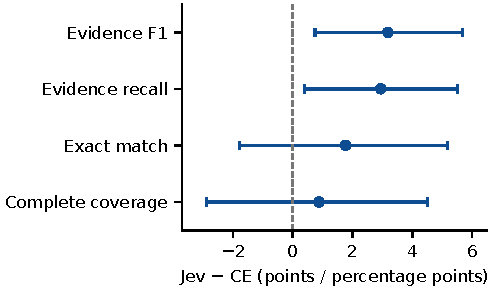
\includegraphics[width=\linewidth]{research/chapter4/figures/section-figures-v1/fig_4_2_evidence_effects_column.pdf}
\caption{최종 근거 성능의 Jev$-$CE 차이와 탐색적 95\% CI. EM·완전 회수율 차이는 \%p, 나머지는 점 단위이다.}
\label{fig:ch4_2}
\end{figure}

F1과 Recall 차이의 CI는 각각 [+0.75, +5.68]점과 [+0.39, +5.51]점이었다(그림 1). 반면 EM은 27.88\%에서 29.65\%로, 모든 gold를 포함한 완전 회수율은 34.07\%에서 34.96\%로 증가하는 데 그쳤다. EM은 선택 집합과 gold 집합의 완전 일치이고, 완전 회수는 정답 외 근거가 있더라도 gold를 빠짐없이 포함한 경우이다. 두 차이의 CI는 0을 포함하였다. 평균적인 근거 회수 수준은 높아졌으나, 필요한 근거를 모두 확보한 문항은 77개에서 79개로 소폭 증가하였다.

문항별 F1은 Jev 우세 32개, 동일 177개, CE 우세 17개였다. 공식 hop별 F1은 1-hop에서 78.07$\to$76.90, 2-hop에서 53.33$\to$57.24, 3-hop에서 47.91$\to$54.83이었다. 이는 집단별 관측 평균이며 효과 차이를 검정한 결과는 아니다. 특히 3-hop 완전 회수는 두 조건 모두 1/42문항이었다. 고유 gold 386개 중 27개는 corpus에서 동일 문자열을 찾을 수 없어 29문항에 영향을 주었다. 완전 매핑 197문항의 F1은 64.12$\to$67.21, 영향 29문항은 20.80$\to$24.71이었다. 전체 분석에서는 이 문항들을 제외하지 않았다.

공개 코드 CE의 F1은 48.72점이었다. 수정 CE와의 9.85점 차이는 후보 목록 참조 수정 효과이며, Jev 교체 효과와 구별된다. 공개 스냅샷의 문제가 원 논문의 실제 실행에도 있었는지는 확인되지 않았다.
